\chapter{HUD}
\label{ch:players/hud}

Mit HUD-Elementen (\emph{Heads-up-Display}) zeigst du Text, Bilder und
andere grafische Elemente an.

Das HUD\index{hud@HUD} nimmt keine Eingaben entgegen; dafür verwendest
du eine
Formspec\index{formspec@Formspec}~(Kapitel~\ref{ch:players/formspecs}).

\begin{hinweis}{type statt hud\_elem\_type}

Seit Luanti 5.9 heißt die Eigenschaft für den Elementtyp \texttt{type}.
Der alte Name \texttt{hud\_\allowbreak{}elem\_\allowbreak{}type}
funktioniert noch, gilt aber als veraltet. Dieses Kapitel verwendet
durchgehend \texttt{type}.

\end{hinweis}

\section{Positionierung}\label{positionierung}

\subsection{Position und Versatz}\label{position-und-versatz}

\begin{figure}
\centering
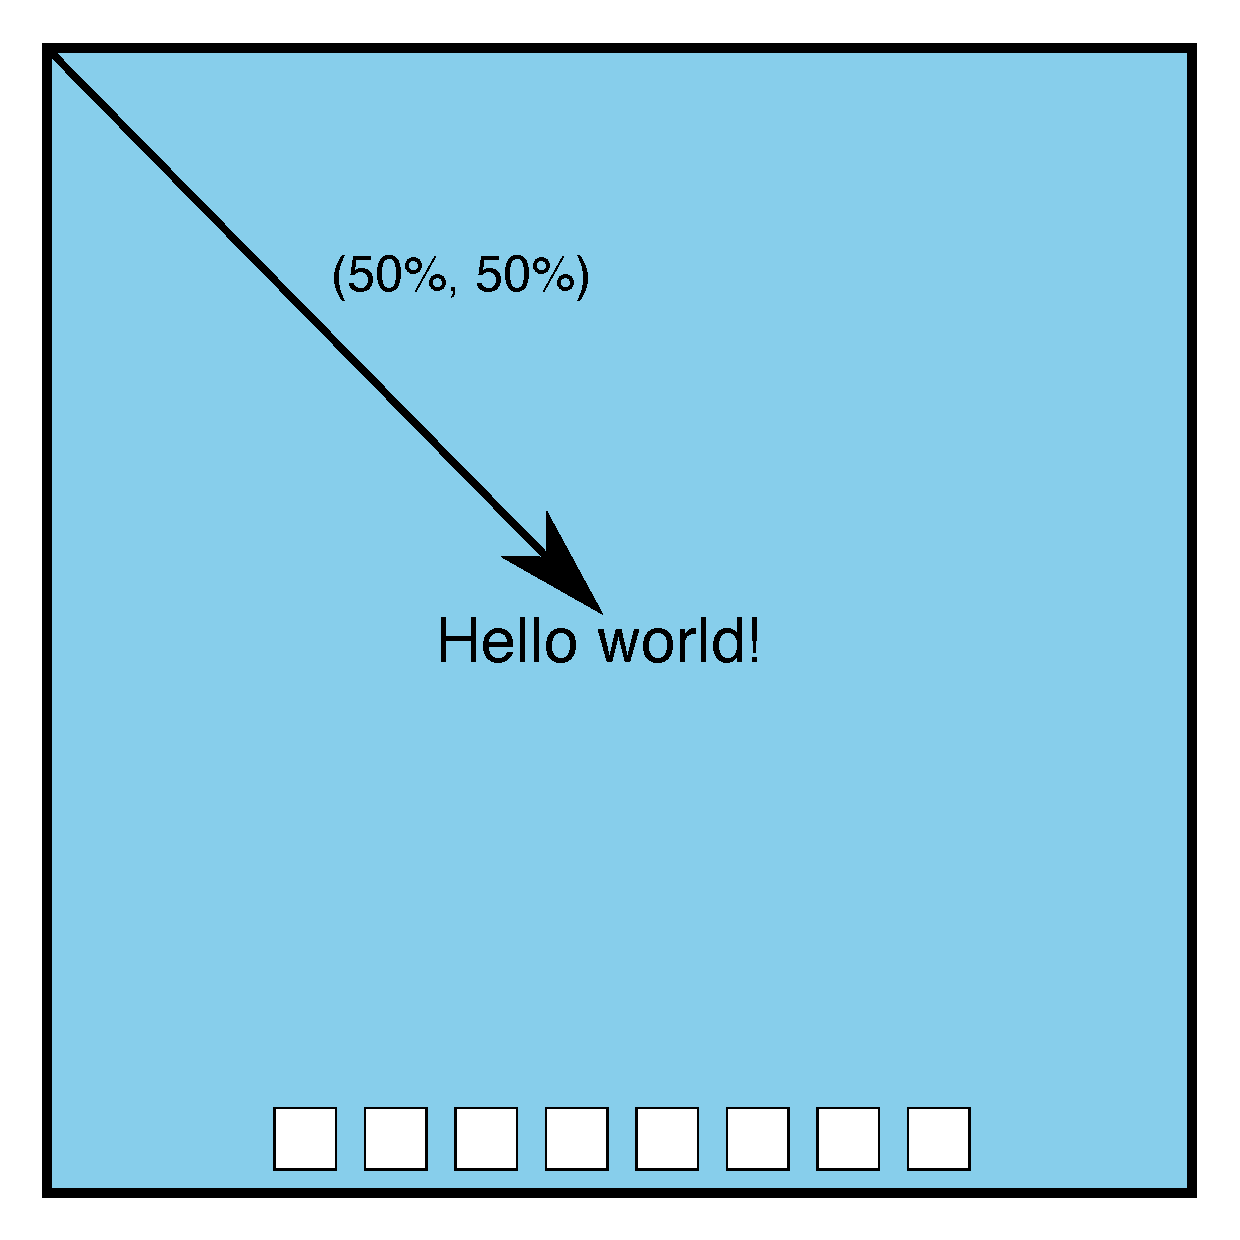
\includegraphics[width=6cm,height=\textheight,keepaspectratio,alt={Ein zentriertes Textelement}]{bilder/hud_diagram_center.pdf}
\caption{Ein zentriertes Textelement}
\end{figure}

Bildschirme gibt es in vielen Größen und Auflösungen, und das HUD muss
auf allen gut funktionieren.

Luanti löst das, indem die Lage eines Elements aus einer prozentualen
Position und einem Versatz (\emph{offset}) bestimmt wird. Die
prozentuale Position bezieht sich auf die Bildschirmgröße. Um ein
Element in der Bildschirmmitte zu platzieren, gibst du also die halbe
Bildschirmgröße als Position an, etwa (50 \%, 50 \%), und einen Versatz
von (0, 0).

Mit dem Versatz verschiebst du das Element dann relativ zur prozentualen
Position.

\subsection{Ausrichtung}\label{ausrichtung}

Die Ausrichtung (\emph{alignment}) legt fest, wo am Element der aus
Position und Versatz berechnete Punkt liegt. Mit
\texttt{\{x = -1.\allowbreak{}0, y = 0.\allowbreak{}0\}} zeigt dieser
Punkt zum Beispiel auf den linken Rand des Elements. Das ist besonders
nützlich, um Text links, mittig oder rechts auszurichten.

\begin{figure}
\centering
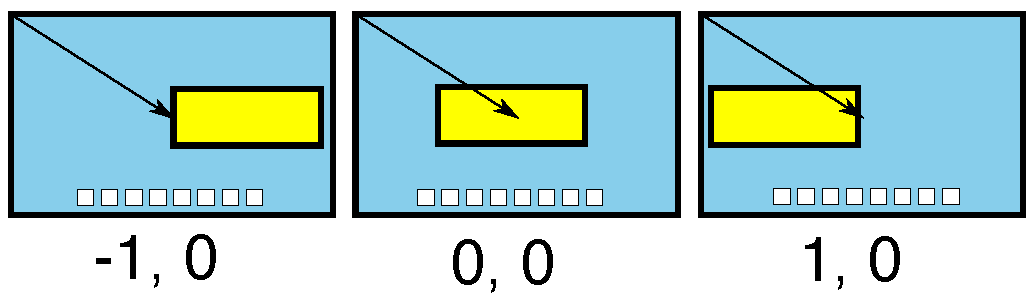
\includegraphics[width=10cm,height=\textheight,keepaspectratio,alt={Ausrichtung}]{bilder/hud_diagram_alignment.pdf}
\caption{Ausrichtung}
\end{figure}

Das Diagramm zeigt drei Fenster (blau) mit jeweils einem HUD-Element
(gelb) und unterschiedlicher Ausrichtung. Der Pfeil ist das Ergebnis aus
Position und Versatz.

\subsection{Punkteanzeige}\label{punkteanzeige}

In diesem Kapitel lernst du, eine Punkteanzeige wie diese zu
positionieren und zu aktualisieren:

\begin{figure}
\centering
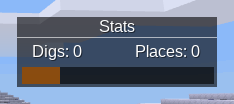
\includegraphics[width=5cm,height=\textheight,keepaspectratio,alt={So soll das HUD am Ende aussehen}]{bilder/hud_final.png}
\caption{So soll das HUD am Ende aussehen}
\end{figure}

Im Bild haben alle Elemente dieselbe prozentuale Position (100 \%, 50
\%), aber unterschiedliche Versätze. So ist das Ganze am rechten
Fensterrand verankert und bleibt beim Ändern der Fenstergröße intakt.

\section{Textelemente}\label{textelemente}

Sobald du das Spielerobjekt hast, kannst du ein HUD-Element anlegen:

\begin{Shaded}
\begin{Highlighting}[]
\KeywordTok{local} \VariableTok{player} \OperatorTok{=} \VariableTok{core}\OperatorTok{.}\NormalTok{get\_player\_by\_name}\OperatorTok{(}\StringTok{"username"}\OperatorTok{)}
\KeywordTok{local} \VariableTok{idx} \OperatorTok{=} \VariableTok{player}\OperatorTok{:}\NormalTok{hud\_add}\OperatorTok{(\{}
    \FunctionTok{type} \OperatorTok{=} \StringTok{"text"}\OperatorTok{,}
    \VariableTok{position} \OperatorTok{=} \OperatorTok{\{} \VariableTok{x} \OperatorTok{=} \DecValTok{0.5}\OperatorTok{,} \VariableTok{y} \OperatorTok{=} \DecValTok{0.5} \OperatorTok{\},}
    \VariableTok{offset} \OperatorTok{=} \OperatorTok{\{} \VariableTok{x} \OperatorTok{=} \DecValTok{0}\OperatorTok{,} \VariableTok{y} \OperatorTok{=} \DecValTok{0} \OperatorTok{\},}
    \VariableTok{text} \OperatorTok{=} \StringTok{"Hallo Welt!"}\OperatorTok{,}
    \VariableTok{alignment} \OperatorTok{=} \OperatorTok{\{} \VariableTok{x} \OperatorTok{=} \DecValTok{0}\OperatorTok{,} \VariableTok{y} \OperatorTok{=} \DecValTok{0} \OperatorTok{\},} \CommentTok{{-}{-} zentriert}
    \VariableTok{scale} \OperatorTok{=} \OperatorTok{\{} \VariableTok{x} \OperatorTok{=} \DecValTok{100}\OperatorTok{,} \VariableTok{y} \OperatorTok{=} \DecValTok{100} \OperatorTok{\},} \CommentTok{{-}{-} siehe unten}
\OperatorTok{\})}
\end{Highlighting}
\end{Shaded}

\texttt{hud\_\allowbreak{}add} gibt eine Element-ID zurück, mit der du
das HUD-Element später ändern oder entfernen kannst.

\subsection{Parameter}\label{parameter}

Den Elementtyp gibst du mit der Eigenschaft \texttt{type} in der
Definitionstabelle an. Die Bedeutung der übrigen Eigenschaften hängt vom
Typ ab.

\texttt{scale} ist der maximale Bereich für den Text; Text außerhalb
wird abgeschnitten, z.~B. \texttt{\{x=100, y=100\}}.

\texttt{number} ist die Textfarbe als Hexadezimalzahl, z.~B.
\texttt{0xFF0000}.

\subsection{Unser Beispiel}\label{unser-beispiel}

Platzieren wir nun alle Texte unserer Punkteanzeige:

\begin{Shaded}
\begin{Highlighting}[]
\CommentTok{{-}{-} Zähler aus dem Speicher holen, Standard 0}
\KeywordTok{local} \VariableTok{meta} \OperatorTok{=} \VariableTok{player}\OperatorTok{:}\NormalTok{get\_meta}\OperatorTok{()}
\KeywordTok{local} \VariableTok{digs\_text} \OperatorTok{=} \StringTok{"Abgebaut: "} \OperatorTok{..} \VariableTok{meta}\OperatorTok{:}\NormalTok{get\_int}\OperatorTok{(}\StringTok{"score:digs"}\OperatorTok{)}
\KeywordTok{local} \VariableTok{places\_text} \OperatorTok{=} \StringTok{"Platziert: "}
    \OperatorTok{..} \VariableTok{meta}\OperatorTok{:}\NormalTok{get\_int}\OperatorTok{(}\StringTok{"score:places"}\OperatorTok{)}

\VariableTok{player}\OperatorTok{:}\NormalTok{hud\_add}\OperatorTok{(\{}
    \FunctionTok{type} \OperatorTok{=} \StringTok{"text"}\OperatorTok{,}
    \VariableTok{position} \OperatorTok{=} \OperatorTok{\{} \VariableTok{x} \OperatorTok{=} \DecValTok{1}\OperatorTok{,} \VariableTok{y} \OperatorTok{=} \DecValTok{0.5} \OperatorTok{\},}
    \VariableTok{offset} \OperatorTok{=} \OperatorTok{\{} \VariableTok{x} \OperatorTok{=} \OperatorTok{{-}}\DecValTok{120}\OperatorTok{,} \VariableTok{y} \OperatorTok{=} \OperatorTok{{-}}\DecValTok{25} \OperatorTok{\},}
    \VariableTok{text} \OperatorTok{=} \StringTok{"Statistik"}\OperatorTok{,}
    \VariableTok{alignment} \OperatorTok{=} \OperatorTok{\{} \VariableTok{x} \OperatorTok{=} \DecValTok{0}\OperatorTok{,} \VariableTok{y} \OperatorTok{=} \DecValTok{0} \OperatorTok{\},}
    \VariableTok{scale} \OperatorTok{=} \OperatorTok{\{} \VariableTok{x} \OperatorTok{=} \DecValTok{100}\OperatorTok{,} \VariableTok{y} \OperatorTok{=} \DecValTok{30} \OperatorTok{\},}
    \VariableTok{number} \OperatorTok{=} \DecValTok{0xFFFFFF}\OperatorTok{,}
\OperatorTok{\})}

\VariableTok{player}\OperatorTok{:}\NormalTok{hud\_add}\OperatorTok{(\{}
    \FunctionTok{type} \OperatorTok{=} \StringTok{"text"}\OperatorTok{,}
    \VariableTok{position} \OperatorTok{=} \OperatorTok{\{} \VariableTok{x} \OperatorTok{=} \DecValTok{1}\OperatorTok{,} \VariableTok{y} \OperatorTok{=} \DecValTok{0.5} \OperatorTok{\},}
    \VariableTok{offset} \OperatorTok{=} \OperatorTok{\{} \VariableTok{x} \OperatorTok{=} \OperatorTok{{-}}\DecValTok{180}\OperatorTok{,} \VariableTok{y} \OperatorTok{=} \DecValTok{0} \OperatorTok{\},}
    \VariableTok{text} \OperatorTok{=} \VariableTok{digs\_text}\OperatorTok{,}
    \VariableTok{alignment} \OperatorTok{=} \OperatorTok{\{} \VariableTok{x} \OperatorTok{=} \OperatorTok{{-}}\DecValTok{1}\OperatorTok{,} \VariableTok{y} \OperatorTok{=} \DecValTok{0} \OperatorTok{\},}
    \VariableTok{scale} \OperatorTok{=} \OperatorTok{\{} \VariableTok{x} \OperatorTok{=} \DecValTok{50}\OperatorTok{,} \VariableTok{y} \OperatorTok{=} \DecValTok{10} \OperatorTok{\},}
    \VariableTok{number} \OperatorTok{=} \DecValTok{0xFFFFFF}\OperatorTok{,}
\OperatorTok{\})}

\VariableTok{player}\OperatorTok{:}\NormalTok{hud\_add}\OperatorTok{(\{}
    \FunctionTok{type} \OperatorTok{=} \StringTok{"text"}\OperatorTok{,}
    \VariableTok{position} \OperatorTok{=} \OperatorTok{\{} \VariableTok{x} \OperatorTok{=} \DecValTok{1}\OperatorTok{,} \VariableTok{y} \OperatorTok{=} \DecValTok{0.5} \OperatorTok{\},}
    \VariableTok{offset} \OperatorTok{=} \OperatorTok{\{} \VariableTok{x} \OperatorTok{=} \OperatorTok{{-}}\DecValTok{70}\OperatorTok{,} \VariableTok{y} \OperatorTok{=} \DecValTok{0} \OperatorTok{\},}
    \VariableTok{text} \OperatorTok{=} \VariableTok{places\_text}\OperatorTok{,}
    \VariableTok{alignment} \OperatorTok{=} \OperatorTok{\{} \VariableTok{x} \OperatorTok{=} \OperatorTok{{-}}\DecValTok{1}\OperatorTok{,} \VariableTok{y} \OperatorTok{=} \DecValTok{0} \OperatorTok{\},}
    \VariableTok{scale} \OperatorTok{=} \OperatorTok{\{} \VariableTok{x} \OperatorTok{=} \DecValTok{50}\OperatorTok{,} \VariableTok{y} \OperatorTok{=} \DecValTok{10} \OperatorTok{\},}
    \VariableTok{number} \OperatorTok{=} \DecValTok{0xFFFFFF}\OperatorTok{,}
\OperatorTok{\})}
\end{Highlighting}
\end{Shaded}

Das ergibt Folgendes:

\begin{figure}
\centering
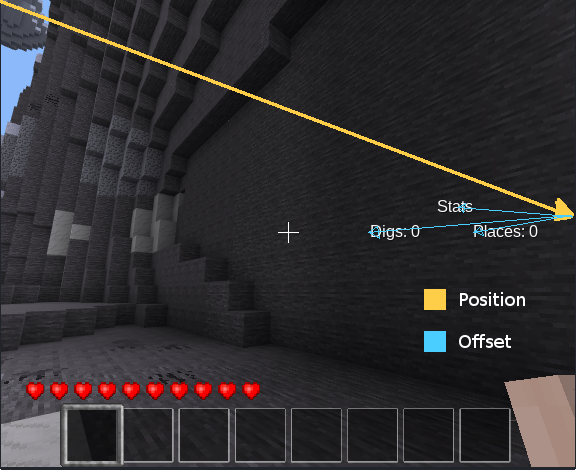
\includegraphics[width=6cm,height=\textheight,keepaspectratio,alt={Die Textelemente der Punkteanzeige}]{bilder/hud_text.png}
\caption{Die Textelemente der Punkteanzeige}
\end{figure}

\section{Bildelemente}\label{bildelemente}

Bildelemente legst du ganz ähnlich an wie Textelemente:

\begin{Shaded}
\begin{Highlighting}[]
\VariableTok{player}\OperatorTok{:}\NormalTok{hud\_add}\OperatorTok{(\{}
    \FunctionTok{type} \OperatorTok{=} \StringTok{"image"}\OperatorTok{,}
    \VariableTok{position} \OperatorTok{=} \OperatorTok{\{} \VariableTok{x} \OperatorTok{=} \DecValTok{1}\OperatorTok{,} \VariableTok{y} \OperatorTok{=} \DecValTok{0.5} \OperatorTok{\},}
    \VariableTok{offset} \OperatorTok{=} \OperatorTok{\{} \VariableTok{x} \OperatorTok{=} \OperatorTok{{-}}\DecValTok{220}\OperatorTok{,} \VariableTok{y} \OperatorTok{=} \DecValTok{0} \OperatorTok{\},}
    \VariableTok{text} \OperatorTok{=} \StringTok{"score\_background.png"}\OperatorTok{,}
    \VariableTok{scale} \OperatorTok{=} \OperatorTok{\{} \VariableTok{x} \OperatorTok{=} \DecValTok{1}\OperatorTok{,} \VariableTok{y} \OperatorTok{=} \DecValTok{1} \OperatorTok{\},}
    \VariableTok{alignment} \OperatorTok{=} \OperatorTok{\{} \VariableTok{x} \OperatorTok{=} \DecValTok{1}\OperatorTok{,} \VariableTok{y} \OperatorTok{=} \DecValTok{0} \OperatorTok{\},}
\OperatorTok{\})}
\end{Highlighting}
\end{Shaded}

Jetzt sieht es so aus:

\begin{figure}
\centering
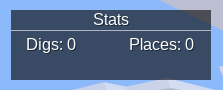
\includegraphics[width=5cm,height=\textheight,keepaspectratio,alt={Die Punkteanzeige mit Hintergrundbild}]{bilder/hud_background_img.png}
\caption{Die Punkteanzeige mit Hintergrundbild}
\end{figure}

\subsection{Parameter}\label{parameter-1}

Im Feld \texttt{text} steht der Name des Bildes.

Ist eine Koordinate von \texttt{scale} positiv, ist sie ein
Skalierungsfaktor: 1 ist die Originalgröße, 2 die doppelte Größe und so
weiter. Ist sie negativ, ist sie ein Prozentwert der Bildschirmgröße;
\texttt{x=-100} bedeutet zum Beispiel 100 \% der Breite.

\subsection{Skalierung}\label{skalierung}

Als Beispiel für die Skalierung bauen wir den Fortschrittsbalken der
Punkteanzeige:

\begin{Shaded}
\begin{Highlighting}[]
\KeywordTok{local} \VariableTok{percent} \OperatorTok{=} \FunctionTok{tonumber}\OperatorTok{(}\VariableTok{meta}\OperatorTok{:}\NormalTok{get}\OperatorTok{(}\StringTok{"score:score"}\OperatorTok{)} \KeywordTok{or} \DecValTok{0.2}\OperatorTok{)}

\VariableTok{player}\OperatorTok{:}\NormalTok{hud\_add}\OperatorTok{(\{}
    \FunctionTok{type} \OperatorTok{=} \StringTok{"image"}\OperatorTok{,}
    \VariableTok{position} \OperatorTok{=} \OperatorTok{\{} \VariableTok{x} \OperatorTok{=} \DecValTok{1}\OperatorTok{,} \VariableTok{y} \OperatorTok{=} \DecValTok{0.5} \OperatorTok{\},}
    \VariableTok{offset} \OperatorTok{=} \OperatorTok{\{} \VariableTok{x} \OperatorTok{=} \OperatorTok{{-}}\DecValTok{215}\OperatorTok{,} \VariableTok{y} \OperatorTok{=} \DecValTok{23} \OperatorTok{\},}
    \VariableTok{text} \OperatorTok{=} \StringTok{"score\_bar\_empty.png"}\OperatorTok{,}
    \VariableTok{scale} \OperatorTok{=} \OperatorTok{\{} \VariableTok{x} \OperatorTok{=} \DecValTok{1}\OperatorTok{,} \VariableTok{y} \OperatorTok{=} \DecValTok{1} \OperatorTok{\},}
    \VariableTok{alignment} \OperatorTok{=} \OperatorTok{\{} \VariableTok{x} \OperatorTok{=} \DecValTok{1}\OperatorTok{,} \VariableTok{y} \OperatorTok{=} \DecValTok{0} \OperatorTok{\},}
\OperatorTok{\})}

\VariableTok{player}\OperatorTok{:}\NormalTok{hud\_add}\OperatorTok{(\{}
    \FunctionTok{type} \OperatorTok{=} \StringTok{"image"}\OperatorTok{,}
    \VariableTok{position} \OperatorTok{=} \OperatorTok{\{} \VariableTok{x} \OperatorTok{=} \DecValTok{1}\OperatorTok{,} \VariableTok{y} \OperatorTok{=} \DecValTok{0.5} \OperatorTok{\},}
    \VariableTok{offset} \OperatorTok{=} \OperatorTok{\{} \VariableTok{x} \OperatorTok{=} \OperatorTok{{-}}\DecValTok{215}\OperatorTok{,} \VariableTok{y} \OperatorTok{=} \DecValTok{23} \OperatorTok{\},}
    \VariableTok{text} \OperatorTok{=} \StringTok{"score\_bar\_full.png"}\OperatorTok{,}
    \VariableTok{scale} \OperatorTok{=} \OperatorTok{\{} \VariableTok{x} \OperatorTok{=} \VariableTok{percent}\OperatorTok{,} \VariableTok{y} \OperatorTok{=} \DecValTok{1} \OperatorTok{\},}
    \VariableTok{alignment} \OperatorTok{=} \OperatorTok{\{} \VariableTok{x} \OperatorTok{=} \DecValTok{1}\OperatorTok{,} \VariableTok{y} \OperatorTok{=} \DecValTok{0} \OperatorTok{\},}
\OperatorTok{\})}
\end{Highlighting}
\end{Shaded}

Jetzt sieht das HUD aus wie das am Anfang des Kapitels! Ein Problem gibt
es allerdings: Es aktualisiert sich nicht, wenn sich die Werte ändern.

\section{Ein Element ändern}\label{ein-element-uxe4ndern}

Mit der ID, die \texttt{hud\_\allowbreak{}add} zurückgibt, kannst du das
Element später ändern oder entfernen.

\begin{Shaded}
\begin{Highlighting}[]
\KeywordTok{local} \VariableTok{idx} \OperatorTok{=} \VariableTok{player}\OperatorTok{:}\NormalTok{hud\_add}\OperatorTok{(\{}
    \FunctionTok{type} \OperatorTok{=} \StringTok{"text"}\OperatorTok{,}
    \VariableTok{text} \OperatorTok{=} \StringTok{"Hallo Welt!"}\OperatorTok{,}
    \CommentTok{{-}{-} weitere Parameter der Kürze halber weggelassen}
\OperatorTok{\})}

\VariableTok{player}\OperatorTok{:}\NormalTok{hud\_change}\OperatorTok{(}\VariableTok{idx}\OperatorTok{,} \StringTok{"text"}\OperatorTok{,} \StringTok{"Neuer Text"}\OperatorTok{)}
\VariableTok{player}\OperatorTok{:}\NormalTok{hud\_remove}\OperatorTok{(}\VariableTok{idx}\OperatorTok{)}
\end{Highlighting}
\end{Shaded}

\texttt{hud\_\allowbreak{}change} erwartet die Element-ID, die zu
ändernde Eigenschaft und den neuen Wert. Der Aufruf oben ändert die
Eigenschaft \texttt{text} von „Hallo Welt!{\kern0pt}`` in „Neuer Text``.

\texttt{hud\_\allowbreak{}change} direkt nach
\texttt{hud\_\allowbreak{}add} aufzurufen, hat also dieselbe Wirkung wie
Folgendes, nur deutlich umständlicher:

\begin{Shaded}
\begin{Highlighting}[]
\KeywordTok{local} \VariableTok{idx} \OperatorTok{=} \VariableTok{player}\OperatorTok{:}\NormalTok{hud\_add}\OperatorTok{(\{}
    \FunctionTok{type} \OperatorTok{=} \StringTok{"text"}\OperatorTok{,}
    \VariableTok{text} \OperatorTok{=} \StringTok{"Neuer Text"}\OperatorTok{,}
\OperatorTok{\})}
\end{Highlighting}
\end{Shaded}

\section{IDs speichern}\label{ids-speichern}

\begin{Shaded}
\begin{Highlighting}[]
\VariableTok{score} \OperatorTok{=} \OperatorTok{\{\}}
\KeywordTok{local} \VariableTok{saved\_huds} \OperatorTok{=} \OperatorTok{\{\}}

\KeywordTok{function} \VariableTok{score}\OperatorTok{.}\NormalTok{update\_hud}\OperatorTok{(}\VariableTok{player}\OperatorTok{)}
    \KeywordTok{local} \VariableTok{player\_name} \OperatorTok{=} \VariableTok{player}\OperatorTok{:}\NormalTok{get\_player\_name}\OperatorTok{()}

    \CommentTok{{-}{-} Zähler aus dem Speicher holen, Standard 0}
    \KeywordTok{local} \VariableTok{meta} \OperatorTok{=} \VariableTok{player}\OperatorTok{:}\NormalTok{get\_meta}\OperatorTok{()}
    \KeywordTok{local} \VariableTok{digs\_text} \OperatorTok{=} \StringTok{"Abgebaut: "}
        \OperatorTok{..} \VariableTok{meta}\OperatorTok{:}\NormalTok{get\_int}\OperatorTok{(}\StringTok{"score:digs"}\OperatorTok{)}
    \KeywordTok{local} \VariableTok{places\_text} \OperatorTok{=} \StringTok{"Platziert: "}
        \OperatorTok{..} \VariableTok{meta}\OperatorTok{:}\NormalTok{get\_int}\OperatorTok{(}\StringTok{"score:places"}\OperatorTok{)}
    \KeywordTok{local} \VariableTok{percent} \OperatorTok{=} \FunctionTok{tonumber}\OperatorTok{(}\VariableTok{meta}\OperatorTok{:}\NormalTok{get}\OperatorTok{(}\StringTok{"score:score"}\OperatorTok{)} \KeywordTok{or} \DecValTok{0.2}\OperatorTok{)}

    \KeywordTok{local} \VariableTok{ids} \OperatorTok{=} \VariableTok{saved\_huds}\OperatorTok{[}\VariableTok{player\_name}\OperatorTok{]}
    \ControlFlowTok{if} \VariableTok{ids} \ControlFlowTok{then}
        \VariableTok{player}\OperatorTok{:}\NormalTok{hud\_change}\OperatorTok{(}
            \VariableTok{ids}\OperatorTok{[}\StringTok{"places"}\OperatorTok{],}
            \StringTok{"text"}\OperatorTok{,}
            \VariableTok{places\_text}
        \OperatorTok{)}
        \VariableTok{player}\OperatorTok{:}\NormalTok{hud\_change}\OperatorTok{(}\VariableTok{ids}\OperatorTok{[}\StringTok{"digs"}\OperatorTok{],} \StringTok{"text"}\OperatorTok{,} \VariableTok{digs\_text}\OperatorTok{)}
        \VariableTok{player}\OperatorTok{:}\NormalTok{hud\_change}\OperatorTok{(}
            \VariableTok{ids}\OperatorTok{[}\StringTok{"bar\_foreground"}\OperatorTok{],}
            \StringTok{"scale"}\OperatorTok{,}
            \OperatorTok{\{} \VariableTok{x} \OperatorTok{=} \VariableTok{percent}\OperatorTok{,} \VariableTok{y} \OperatorTok{=} \DecValTok{1} \OperatorTok{\}}
        \OperatorTok{)}
    \ControlFlowTok{else}
        \VariableTok{ids} \OperatorTok{=} \OperatorTok{\{\}}
        \VariableTok{saved\_huds}\OperatorTok{[}\VariableTok{player\_name}\OperatorTok{]} \OperatorTok{=} \VariableTok{ids}

        \CommentTok{{-}{-} HUD{-}Elemente anlegen, IDs in \textasciigrave{}ids\textasciigrave{} merken}
    \ControlFlowTok{end}
\KeywordTok{end}

\VariableTok{core}\OperatorTok{.}\NormalTok{register\_on\_joinplayer}\OperatorTok{(}\VariableTok{score}\OperatorTok{.}\VariableTok{update\_hud}\OperatorTok{)}

\VariableTok{core}\OperatorTok{.}\NormalTok{register\_on\_leaveplayer}\OperatorTok{(}\KeywordTok{function}\OperatorTok{(}\VariableTok{player}\OperatorTok{)}
    \VariableTok{saved\_huds}\OperatorTok{[}\VariableTok{player}\OperatorTok{:}\NormalTok{get\_player\_name}\OperatorTok{()]} \OperatorTok{=} \KeywordTok{nil}
\KeywordTok{end}\OperatorTok{)}
\end{Highlighting}
\end{Shaded}

\section{Weitere Elemente}\label{weitere-elemente}

Eine vollständige Liste der HUD-Elemente findest du in der
Lua-API-Referenz\footnote{\url{https://api.luanti.org/hud/}}.
